\documentclass[11pt]{article}
\usepackage{amsmath}
\usepackage{graphicx}
\usepackage{float}
\usepackage{blindtext}
\usepackage{subcaption}
\usepackage[a4paper,margin=2cm]{geometry}
\usepackage{fancyhdr}
\usepackage{longtable}
\usepackage[
    backend=biber,
    style=ieee
]{biblatex}
\usepackage{xcolor}
\usepackage{soul}

\newcommand{\hlc}[2][yellow]{{%
    \colorlet{foo}{#1}%
    \sethlcolor{foo}\hl{#2}}%
}

\addbibresource{report.bib}

\graphicspath{ {./images/} }

\pagestyle{fancy}
\fancyhead[C]{Report}
\fancyhead[L]{EEE3032 Visual Search Project}
\fancyhead[R]{22nd of November}

\cfoot{} % get rid of the page number 
\fancyfoot[L]{6596386}
\fancyhead[C]{}
\fancyfoot[R]{\thepage}

\begin{document}
\begin{titlepage}
    \begin{center}
    
\includegraphics[width=\textwidth]{Logo.png} % also works with logo.pdf
    \vfill
    \Huge
    \textbf{EEE3027: Multiplier Assignment}
    \vfill
    \huge
    Assignment Report\\
    \vspace{1cm}
    \Large
    14th of March 2023\\
    URN: 6596386\\
    \vfill
    \vfill
    \Large
    Department of Electronic Engineering\\
    Faculty of Engineering and Physical Sciences\\
    University of Surrey\\
    \end{center}
\end{titlepage}

\begin{abstract}
A report init

\vspace{1cm}
\end{abstract}
\tableofcontents
\pagebreak

\section{8-Bit Multiplier}
For this assignment the components for this style of multiplier were provided.
This includes an 8-bit ripple adder, an 8-bit register, an 8-bit multiplexer, a variable length zero detector, a variable length shift register, a Moore state machine,
and the design for the 8-bit multiplier.
Note that this final design is structural, with the VHDL code for the multiplier only connecting components together.


\subsection{Theory}
The core operation of multiplying two numbers, regardless of base, is to 
multiply the digits, add the product to a total, and then shift the originals numbers\cite{dally}.
This process can be visualized using "long multiplication" as below ($4_{16} \times D_{16}$):
\begin{equation}
    \begin{tabular}{c c c c c c c c c }
                &   &   &   &   & 0 & 1 & 0 & 0 \\
                &   &   &   &  $\times$ & 1 & 1 & 0 & 1 \\
                \hline
                &   &   &   &   & 0 & 1 & 0 & 0 \\
                &   &   &   & 0 & 0 & 0 & 0 &   \\
                &   &   & 0 & 1 & 0 & 0 &   &   \\
                &   & 0 & 1 & 0 & 0 &   &   &   \\
                \hline
                & 0 & 0 & 1 & 1 & 0 & 1 & 0 & 0 \\
    \end{tabular} 
\end{equation}

For the first step of multiplication binary offers an advantage over other bases as only 4 cases need to be considered: 
$0 \times 0 = 0$, $1 \times 0 = 0$, $0 \times 1 = 0$, and $1 \times 1 = 1$ (this matches the truth table of an AND gate).
To then add this product full adders can be employed.
Shifting is the act of multiplying or dividing a number by its base, in the case of binary that is two.
In practice this can be moving the connections in opposite directions after each multiply and add. 
This basic theory will lead us to the combinational design in figure \ref{fig:mult_fa}.

\begin{figure}[H]        
    \centering
    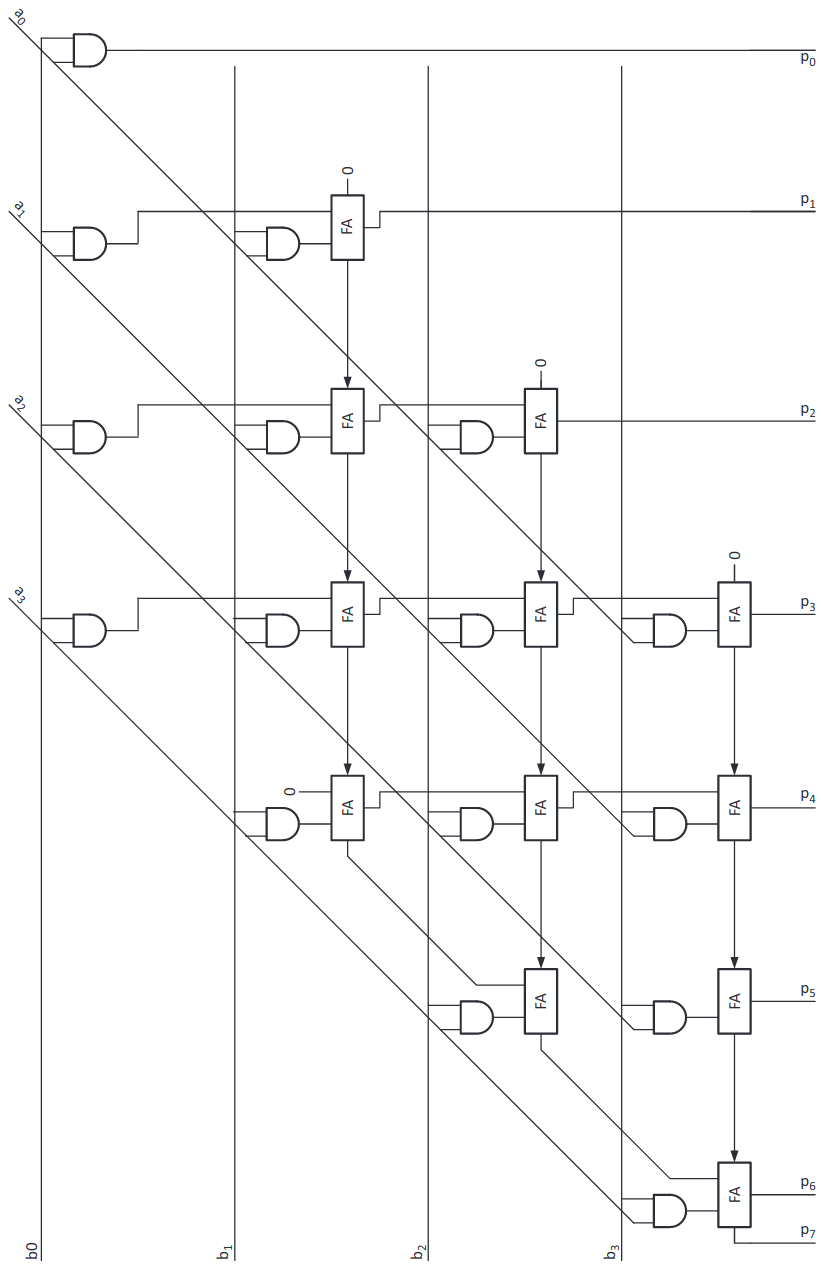
\includegraphics[width=.5\textwidth]{MultFA.png}
    \caption{8-Bit Multiplier using Full Adders \cite{dally}}
    \label{fig:mult_fa}
\end{figure} 

The multiplier achieves all the steps requires as can be seen moving colum to colum. 
In the first colum multiplication occurs using AND gates.
Then all the inputs get shifted over, as can be seen by the AND gates moving down and the diagonal lines for the A input followed by another multiply and add.
This continues, ensuring the carry term also get forwarded appropriately until the output is achieved.

\subsubsection{State Machine Multiplier}

For this assignment however this combinational design was not used, 
instead a sequential style of multiplier was provided which is clocked and relies on a Moore state machine to control shifting and adding.
Unlike in combinational circuits, which rely only on the current state of the input, sequential designs use feedback to store information about previous inputs\cite{dally}.
In this case the given circuit is also synchronous meaning that any storage is linked to a clock to ensure all changes happen simultaneously and that races do not occur.
Being both sequential and synchronous makes our circuit a Finite-State Machine\cite{dally}.
Figure \ref{fig:4bit_mult} shows this alternative multiplier design. 

\begin{figure}[H]        
    \centering
    
\includegraphics[width=.5\textwidth]{Logo.png}
    \caption{8-Bit Multiplier using State Machine}
    \label{fig:4bit_mult}
\end{figure} 

F1, our state machine, is at the core of this design and in order to understand the multiplier the operation of the state machine must be understood.
One way to visualize a state machine is with a state diagram, such as the one in figure \ref{fig:msm} which is based on the design in \cite{smith1997application}.

\begin{figure}[H]        
    \centering
    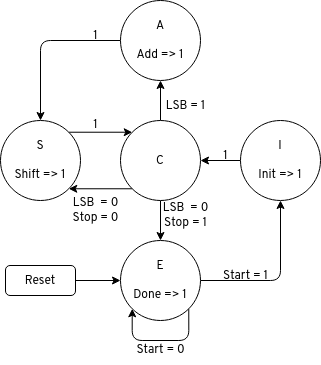
\includegraphics[width=.5\textwidth]{StateMachine.png}
    \caption{Moore State Machine for Multiplier}
    \label{fig:msm}
\end{figure} 

Upon reset we will always enter state E,
this is also in fact the only asynchronous part of the design as this state change will happen as soon as the reset lines goes high while every other state change will only occur on the rising edge of the clock.
In state E the state machine will output '1' on the Done line (any output not labeled as going to '1' is assumed to go to '0') which does not impact any of the other components and is in fact simply and output of the multiplier.
As shown in the diagram while in state E every clock the start signal is checked, as long as it it '0' the state machine remains in state E however once it is high it moves to state I.
State I takes the Init line to '1', when tracing this line it can be seen that the following event will occur simultaneously: OR gate REGclr is given an input meaning the gate's output will go to '1' clearing the register of any previous values on the next rising edge.
Note that this will also happen when the Reset line goes high as it connects to the other input of the OR gate. 
The Init line also connects to the LD of both shift registers causing inputs A and B to load into shift registers SR1 and SR2 respectively on the next rising edge.
Once in the I state the state machine will always transition to state C. 
In state C the machine "checks" the value of shift register SR1,
in particular if all the bits of SR1's output bus are zero (which is sent by the all zero detect Z1 into the stop line) as well as the value of the least significant bit (LSB).
If the LSB bit is '1' we move to the A state, otherwise the stop line is checked.
When the stop line and LSB bit are '0' the S state is selected and finally if the stop line is '1' and the LSB is '0' we return to the E state.
When in the A state the Add lines goes to '1', which will make the multiplexer M1 select the output of adder A1 instead of the current value of the register R1.
R1 hold the output value meaning that when the Add line is '0' and M1 feed R1 back into R1 nothing will happen, however when R1 is high the output of A1 will be go into R1.
A1 adds the output of SR2 together with R1.
State A will always transition to state S which takes the Shift line to '1', causing both SR1 and SR2 to shift with SR1 shifting right as DIR is taken low and SR2 shifting left as DIR is taken high.
Then state S will transition to state C.

These three states C, A, and S are the core of the multiplying operation and mirror the steps outlined earlier for multiplying binary numbers.
Instead of directly multiplying two 4-bit numbers this state machine break the multiplication into multiple 4-bit by 1-bit multiplications.
For any N-bit ($n$) by 1-bit ($b$) multiplication the following holds: $n \times b = n$ if $b = 1$ or $n \times b = 0$ if $b = 0$.
So the way the state machine multiplies two multi-bit binary numbers $A$ and $B$ a shifted copy of $B$ is added for every position $A$ is 1\cite{dally}. 
The shifts form state S will make the LSB the next bit of A and will shift up B at the same time.
Once A is all zeros the state machines goes to the end state as no more adding is required. 

\subsection{Test Bench}
The provided test bench code for the 8-bit multiplier was used with some minor changes and corrections.
The initially provided code used SRA as a variable name which is invalid VHDL code as SRA is in the reserved list,
this however is a simple fix as the variable can renamed throughout the test bench.
In order to make the test bench more thorough the range of values investigated was increased to cover very possible 4-bit input (0 to 255) instead of the original limited range,
this made finding errors more complicated however due to the large amount of values so another signal was added that keeps a running total of the amount of errors.
The error checking is done with an if statement that compares the product of the integer in the for loops to the output out multiplier,
if the values do no match an error is logged and the error count in incremented. 
Keeping track of errors helped during debugging to ensure that the multiplier functioned as expected. 

\begin{figure}[H]        
    \centering
    
\includegraphics[width=.5\textwidth]{Logo.png}
    \caption{Test Bench of 8-Bit Multiplier}
    \label{fig:4bit_testbench}
\end{figure} 

Comprehensive testing ensures

\subsection{Timing Analysis}

The worst case timing of the 8-bit multiplier can be found by delving into state machine. 
This is because timing is dictated by the amount of clock cycles, with each full clock cycle being 20ns, and the state machine will dictated how many clock cycles multiplication takes.
Referring to the diagram in figure \ref{fig:msm} the shortest journey occurs when we go from $E \rightarrow I \rightarrow C \rightarrow E$, which occurs anytime A is $A = 0_16$ regardless of the value of B.
This would take only 60ns to from start input to done output.
The longest journey will occur if we need to add and shift for every single bit of A, ie when $A = F_16$, this is once again independent of the value of B.
In this case we would go $E \rightarrow I \rightarrow C \rightarrow A \rightarrow S \rightarrow C \rightarrow A \rightarrow S \rightarrow C \rightarrow A \rightarrow S \rightarrow C \rightarrow A \rightarrow S \rightarrow C \rightarrow E$.
This would take 300ns from start to done, which we can confirm in simulation as seen in figure \ref{fig:4bit_worstcase}.

\begin{figure}[H]        
    \centering
    
\includegraphics[width=.5\textwidth]{Logo.png}
    \caption{Worst Case performance of 8-Bit Multiplier}
    \label{fig:4bit_worstcase}
\end{figure} 

\section{8-Bit Multiplier}

8-Bit multipliers can be constructed in various methods, one simple example would be expanding the design seen in figure \ref{fig:mult_fa} to take 8-bit inputs and to extend the shift-registers, register, multiplexer and adder in figure \ref{fig:4bit_mult}.
These methods however go against some VHDL good practice (as well as against the assignment's instructions),
as it is preferred to have smaller components that can be reused throughout a design.

Instead therefore the 8-bit multiplier was used as a component, along side more 8-bit adders. 
This is because we can describe 16-bit multiplication as four separate 8-bit multiplication.
Take for example the multiplication of $49_16$ and $9D_16$ in equation \ref{eq:16bit} below.

\begin{equation}
    \label{eq:16bit}
    \begin{tabular}{c c c c c c c c c c c c c c c c c c}
        &   &   &   &   &  &  &  &   & 0 & 1 & 0 & 0 & 1 & 0 & 0 & 1\\
        &   &   &   & &&&&$\times$   & 1 & 0 & 0 & 1 & 1 & 1 & 0 & 1 \\
                \hline
        &   &   &   &   &   &   &   &   & \hlc[cyan]{0} & \hlc[cyan]{1} & \hlc[cyan]{0} & \hlc[cyan]{0} & \hlc[yellow]{1} & \hlc[yellow]{0} & \hlc[yellow]{0} & \hlc[yellow]{1} \\
        &   &   &   &   &   &   &   & \hlc[cyan]{0} & \hlc[cyan]{0} & \hlc[cyan]{0} & \hlc[cyan]{0} & \hlc[yellow]{0} & \hlc[yellow]{0} & \hlc[yellow]{0} & \hlc[yellow]{0} &   \\
        &   &   &   &   &   &   & \hlc[cyan]{0} & \hlc[cyan]{1} & \hlc[cyan]{0} & \hlc[cyan]{0} & \hlc[yellow]{1} & \hlc[yellow]{0} & \hlc[yellow]{0} & \hlc[yellow]{1} &   &   \\
        &   &   &   &   &   & \hlc[cyan]{0} & \hlc[cyan]{1} & \hlc[cyan]{0} & \hlc[cyan]{0} & \hlc[yellow]{1} & \hlc[yellow]{0} & \hlc[yellow]{0} & \hlc[yellow]{1} &   &   &   \\
        &   &   &   &   & \hlc[green]{0} & \hlc[green]{1} & \hlc[green]{0} & \hlc[green]{0} & \hlc[pink]{1} & \hlc[pink]{0} & \hlc[pink]{0} & \hlc[pink]{1} &   &   &   &   \\
        &   &   &   & \hlc[green]{0} & \hlc[green]{0} & \hlc[green]{0} & \hlc[green]{0} & \hlc[pink]{0} & \hlc[pink]{0} & \hlc[pink]{0} & \hlc[pink]{0} &   &   &   &   &   \\
        &   &   & \hlc[green]{0} & \hlc[green]{0} & \hlc[green]{0} & \hlc[green]{0} & \hlc[pink]{0} & \hlc[pink]{0} & \hlc[pink]{0} & \hlc[pink]{0} &   &   &   &   &   &   \\
        &   & \hlc[green]{0} & \hlc[green]{1} & \hlc[green]{0} & \hlc[green]{0} & \hlc[pink]{1} & \hlc[pink]{0} & \hlc[pink]{0} & \hlc[pink]{1} &   &   &   &   &   &   &   \\
                \hline
        & 0 & 0 & 1 & 0 & 1 & 1 & 0 & 0 & 1 & 1 & 0 & 0 & 0 & 1 & 0 & 1 \\
    \end{tabular} 
\end{equation}

As shown by the colors this can be broken down into the following four 8-bit multiplications. 
\vspace{5mm}
\begin{minipage}{.5\linewidth}
    \begin{equation}
        \label{eq:yellow}
        \begin{tabular}{c c c c c c c c c }
            &   &   &   &   & 1 & 0 & 0 & 1 \\
            &   &   &   &  $\times$ & 1 & 1 & 0 & 1 \\
            \hline
            &   &   &   &   & 1 & 0 & 0 & 1 \\
            &   &   &   & 0 & 0 & 0 & 0 &   \\
            &   &   & 1 & 0 & 0 & 1 &   &   \\
            &   & 1 & 0 & 0 & 1 &   &   &   \\
            \hline
            & \hlc[yellow]{0} & \hlc[yellow]{1} & \hlc[yellow]{1} & \hlc[yellow]{1} & \hlc[yellow]{0} & \hlc[yellow]{1} & \hlc[yellow]{0} & \hlc[yellow]{1} \\
        \end{tabular} 
    \end{equation}
    \end{minipage}%
    \begin{minipage}{.5\linewidth}
        \begin{equation}
            \label{eq:blue}
            \begin{tabular}{c c c c c c c c c }
                &   &   &   &   & 0 & 1 & 0 & 0 \\
                &   &   &   &  $\times$ & 1 & 1 & 0 & 1 \\
                \hline
                &   &   &   &   & 0 & 1 & 0 & 0 \\
                &   &   &   & 0 & 0 & 0 & 0 &   \\
                &   &   & 0 & 1 & 0 & 0 &   &   \\
                &   & 0 & 1 & 0 & 0 &   &   &   \\
                \hline
                & \hlc[cyan]{0} & \hlc[cyan]{0} & \hlc[cyan]{1} & \hlc[cyan]{1} & \hlc[cyan]{0} & \hlc[cyan]{1} & \hlc[cyan]{0} & \hlc[cyan]{0} \\
            \end{tabular} 
        \end{equation}
\end{minipage}
\vspace{5mm}
\begin{minipage}{.5\linewidth}
    \begin{equation}
        \label{eq:pink}
        \begin{tabular}{c c c c c c c c c }
            &   &   &   &   & 1 & 0 & 0 & 1 \\
            &   &   &   &  $\times$ & 1 & 0 & 0 & 1 \\
            \hline
            &   &   &   &   & 1 & 0 & 0 & 1 \\
            &   &   &   & 0 & 0 & 0 & 0 &   \\
            &   &   & 0 & 0 & 0 & 0 &   &   \\
            &   & 1 & 0 & 0 & 1 &   &   &   \\
            \hline
            & \hlc[pink]{0} & \hlc[pink]{1} & \hlc[pink]{0} & \hlc[pink]{1} & \hlc[pink]{0} & \hlc[pink]{0} & \hlc[pink]{0} & \hlc[pink]{1} \\
        \end{tabular} 
    \end{equation}
    \end{minipage}%
    \begin{minipage}{.5\linewidth}
        \begin{equation}
            \label{eq:green}
            \begin{tabular}{c c c c c c c c c }
                &   &   &   &   & 0 & 1 & 0 & 0 \\
                &   &   &   &  $\times$ & 1 & 0 & 0 & 1 \\
                \hline
                &   &   &   &   & 0 & 1 & 0 & 0 \\
                &   &   &   & 0 & 0 & 0 & 0 &   \\
                &   &   & 0 & 0 & 0 & 0 &   &   \\
                &   & 0 & 1 & 0 & 0 &   &   &   \\
                \hline
                & \hlc[green]{0} & \hlc[green]{0} & \hlc[green]{1} & \hlc[green]{0} & \hlc[green]{0} & \hlc[green]{1} & \hlc[green]{0} & \hlc[green]{0} \\
            \end{tabular} 
        \end{equation}
\end{minipage}

The products of these multipliers can then be added together as seen in equation \ref{eq:16bit_add} to get the same result as equation \ref{eq:16bit}.
This addition can achieved with three 16-bit adders, which could be constructed out of six of the provided 8-bit adders.

\begin{equation}
    \label{eq:16bit_add}
    \begin{tabular}{c c c c c c c c c c c c c c c c c c}
        &   &   &   &   &   &   &   & \hlc[yellow]{0} & \hlc[yellow]{1} & \hlc[yellow]{1} & \hlc[yellow]{1} & \hlc[yellow]{0} & \hlc[yellow]{1} & \hlc[yellow]{0} & \hlc[yellow]{1} & \\
        &   &   &   &  \hlc[cyan]{0} & \hlc[cyan]{0} & \hlc[cyan]{1} & \hlc[cyan]{1} & \hlc[cyan]{0} & \hlc[cyan]{1} & \hlc[cyan]{0} & \hlc[cyan]{0}&   &   &   &   &   &\\
        &   &   &   &  \hlc[pink]{0} & \hlc[pink]{1} & \hlc[pink]{0} & \hlc[pink]{1} & \hlc[pink]{0} & \hlc[pink]{0} & \hlc[pink]{0} & \hlc[pink]{1}&  &   &   &   &   \\
        \hlc[green]{0} & \hlc[green]{0} & \hlc[green]{1} & \hlc[green]{0} & \hlc[green]{0} & \hlc[green]{1} & \hlc[green]{0} & \hlc[green]{0}  &   &   &  &   &   &   &   \\
        \hline
        0 & 0 & 1 & 0 & 1 & 1 & 0 & 0 & 1 & 1 & 0 & 0 & 0 & 1 & 0 & 1 & \\

    \end{tabular} 
\end{equation}

\begin{equation}
    \label{eq:16bit_add1}
    \begin{tabular}{c c c c c c c c c }
                &   &   &   &   & \hlc[yellow]{0} & \hlc[yellow]{1} & \hlc[yellow]{1} & \hlc[yellow]{1} \\
            +   & \hlc[cyan]{0} & \hlc[cyan]{0} & \hlc[cyan]{1} & \hlc[cyan]{1} & \hlc[cyan]{0} & \hlc[cyan]{1} & \hlc[cyan]{0} & \hlc[cyan]{0} \\
                \hline
                & 0 & 0 & 1 & 1 & 1 & 0 & 1 & 1 \\
    \end{tabular} 
\end{equation}

\begin{equation}
    \label{eq:16bit_add2}
    \begin{tabular}{c c c c c c c c c c}
                & 0 & 0 & 1 & 1 & 1 & 0 & 1 & 1 \\
               + & \hlc[pink]{0} & \hlc[pink]{1} & \hlc[pink]{0} & \hlc[pink]{1} & \hlc[pink]{0} & \hlc[pink]{0} & \hlc[pink]{0} & \hlc[pink]{1} \\
                \hline
               0 & 1 & 0 & 0 & 0 & 1 & 1 & 0 & 0 \\
    \end{tabular} 
\end{equation}

\begin{equation}
    \label{eq:16bit_add3}
    \begin{tabular}{c c c c c c c c c }
                &   &   &   & 0 & 1 & 0 & 0 & 0 \\
            +   & \hlc[green]{0} & \hlc[green]{0} & \hlc[green]{1} & \hlc[green]{0} & \hlc[green]{0} & \hlc[green]{1} & \hlc[green]{0} & \hlc[green]{0} \\
                \hline
                & 0 & 0 & 1 & 0 & 1 & 1 & 0 & 0 \\
    \end{tabular} 
\end{equation}

However a more efficient design can be created as each of the inputs are "shifted" 8-bit values,
this design makes use of only three 8-bit adders and the operation behind it can be seen in equations \ref{eq:16bit_add1},  \ref{eq:16bit_add2}, and  \ref{eq:16bit_add3}.

Equation \ref{eq:16bit_add} shows how the 3 down to 0 bits of the yellow (\ref{eq:yellow}) multiplier's output can be passed directly into the 3 down to 0 bits of the final results.
The 7 down to 4 bits of this output however have to be summed with the output of the blue (\ref{eq:blue}), but these cannot be directly added as the upper yellow bits have to be shifted down.
This shift can be achieved by wiring the 7 to 4 bits of the yellow to 3 down to 0 inputs of the adders input and keeping the other bits at '0'.
The output of this first adder can then be feed into the next adder along with the pink (\ref{eq:pink}) multiplier product to get the next step as seen in equation \ref{eq:16bit_add2}.
Once more the 3 down to 0 bits can be passed to the final result (the 7 down to 4 bits) and then the 'shifting' can employed once more to shift the 7 down to 4 bits into the 3 down to 0 bits of the next adders input.
Those shifted bits along with the final green multiplier output can be added together in the final third adder as seen in equation \ref{eq:16bit_add3} to product the last 8 bits of the result.

Doing so introduces a few edge cases however as adders also output a carry line. 
For adder 1 the carry can be ignored as the largest output of an 8-bit multiplier is $E1_{16}$,
and accounting for the shift, the largest values the adder will encounter are $0E_{16} + E1_{16}$ for which the output is $EF_{16}$. 
$EF_{16}$ can be conveyed as an 8-bit number meaning the carry will always be '0'.
This however is not true for the adder 2 (\ref{eq:16bit_add2}) where the largest possible sum is $EF_{16} + E1_{16} = 1D0_{16}$, which means the carry line may go to '1'.
Adder 2's carry therefore needs to be propagated, which can be done by connecting it to bit 4 of the adder 3's input,
specifically the input with the down shifted number as bits 7 to 4 will always go unused otherwise.
Adder 3's carry will also always be '0' as the largest possible values to enter this adder would be $1D_{16} + E1_{16} = FE_{16}$, once more a number that can be conveyed in 8-bits.
With all of these steps a 16-bit Multiplier can be constructed out of four 8-bit multipliers and three 8-bit adders. 


\begin{figure}[H]         
    \centering
    
\includegraphics[width=.5\textwidth]{Logo.png}
    \caption{16-Bit Multiplier}
    \label{fig:8bit}
\end{figure} 

The final 16-bit multiplier design can be seen in figure 

\subsection{Theory}
\subsection{Test Bench}
\subsection{Timing Analysis}

\section{Conclusion}

\printbibliography

\end{document}